\section{Scope and inferential framework}
\label{sec:litreview:framework}

Understanding how children acquire language from limited experience is a central problem in developmental science, but the relevant learning conditions cannot be manipulated freely in children. Researchers cannot randomly assign infants to radically different linguistic environments, control the timing of every construction they hear, or intervene directly on the learning architecture they bring to the task. Computational models complement observational and experimental work because they instantiate explicit learning hypotheses and can be exposed to controlled input. In this role, a model can address a learnability question: whether a specified learning procedure is sufficient to acquire a target pattern from a specified body of experience \citep{Chater2008,Perfors2011,dupoux2018cognitive}.

This logic predates contemporary large language models. Early connectionist models were deliberately constructed as cognitive simulations and used to test whether apparently rule-governed behavior could emerge from pattern learning \citep{RumelhartMcClelland1986,Elman1990}. Recurrent networks were subsequently used to study phenomena such as agreement and auxiliary inversion under distributional learning accounts \citep{Elman1991,Lewis2001,Reali2004}. Modern language models differ in an important respect: they are generally optimized for engineering objectives, trained on large collections of adult-written text, and not designed as process models of development \citep{Brown2020,Warstadt2022}. Their strong performance on syntactic, semantic, and reasoning benchmarks is therefore scientifically suggestive, but it does not by itself establish that they learn as children do \citep{Linzen2021,Mahowald2024}.

The inference from a successful simulation is asymmetric. If a model learns a phenomenon under conditions that adequately approximate the child's learning problem, its success provides evidence of \emph{sufficiency}: the represented input and learning biases can, in principle, produce the observed outcome. Failure is less decisive. It may reveal an inadequate learning mechanism, but it may instead arise from missing modalities, an unsuitable objective, an inappropriate evaluation, or input unlike that available to the child. Human learners may also exploit working-memory constraints, perceptual grounding, or social scaffolding that the model does not represent \citep{Tomasello2003,Warstadt2022,Wilcox2024}. A model failure consequently does not establish that a phenomenon is unlearnable from experience, nor does model success establish mechanistic identity.

This chapter develops a calibrated-comparison framework around two necessary dimensions. \emph{Outcome alignment} asks whether the model and the child are evaluated on the same construct, using stimuli, response contrasts, and developmental summaries that support a common interpretation. \emph{Input alignment} asks whether the model's training experience approximates child-available input in amount, register, modality, interactional structure, and temporal organization. The two dimensions are related but not interchangeable. A model trained on child-directed speech but evaluated only by an engineering benchmark provides little direct evidence about child behavior. Conversely, a model tested with developmental stimuli after training on web-scale adult text answers a different learnability question from the one faced by a child.

Architecture is treated here as an experimental variable, not as a third quantity that can be matched by inspection. At Marr's algorithmic level, recurrent, attentional, multimodal, and retrieval-augmented systems embody different hypotheses about memory, representation, and inductive bias \citep{Marr1982,Portelance2024}. Yet there is no independently validated specification of the algorithm used by the developing child against which an architecture can simply be checked. Architectural comparisons become interpretable when input and outcomes are held sufficiently constant: a systematic difference can then identify which properties are sufficient or insufficient under those conditions. Claims of architectural plausibility made before these controls remain underdetermined.

The review is organized by the methodological decisions that determine those inferences. Section~\ref{sec:litreview:outcome} examines task affordances, categorical and graded metrics, developmental trajectories, and measurement uncertainty. Section~\ref{sec:litreview:input} examines the quality, quantity, and temporal organization of model input. Section~\ref{sec:litreview:implications} then states reporting requirements and identifies the empirical gaps addressed by the remainder of this thesis. The review is concept-driven and selective rather than a systematic or meta-analytic census. The study tables therefore map representative paradigms across domains; they should not be read as exhaustive inventories of every developmental experiment or model benchmark.


\section{Outcome alignment}
\label{sec:litreview:outcome}

\subsection{Task affordances across linguistic domains}
\label{sec:litreview:task-affordances}

Outcome alignment is stronger than topical similarity. Giving a child and a model stimuli about ``syntax'' is not sufficient if the child's dependent variable indexes preference after familiarization while the model's score is the probability of an isolated sentence. A calibrated comparison should specify at least four correspondences: the linguistic construct being probed, the information available in the stimulus, the decision or response that produces the dependent variable, and the point in development or training at which it is observed. Where any one of these changes, the interpretation must be qualified.

Child competence is usually inferred through an overt behavior---sucking rate, head turning, visual fixation, pointing, or production---after sensory encoding, attention, decision making, and motor execution. A model usually exposes a probability or hidden representation, which is converted into an experimental outcome by an additional \emph{task model}: a distance function, probe, classifier, prompting protocol, or scoring rule. The task model is part of the hypothesis. Layer choice, pooling, prompt wording, and decision threshold can change the apparent competence even when the underlying trained model is fixed. Table~\ref{tab:litreview:alignment} uses four deliberately conservative alignment categories: \emph{close} when matched stimuli and decisions permit trial-level comparison; \emph{partial} when construct and contrast are shared but response generation differs; \emph{indirect} when only a broader theoretical construct is shared; and \emph{none established} when the literature lacks a defensible counterpart.

\begingroup
\small
\setlength{\tabcolsep}{3.5pt}
\setlength{\LTleft}{0pt}
\setlength{\LTright}{0pt}
\begin{longtable}{@{}p{0.12\textwidth}p{0.25\textwidth}p{0.25\textwidth}p{0.11\textwidth}p{0.21\textwidth}@{}}
\caption[Alignment of developmental and model evaluation]{Alignment of representative developmental and model evaluation paradigms. Ratings describe the current measurement correspondence, not the importance of the linguistic domain.}\label{tab:litreview:alignment}\\
\toprule
\textbf{Domain} & \textbf{Child measure} & \textbf{Model measure} & \textbf{Alignment} & \textbf{Representative evidence} \\
\midrule
\endfirsthead
\multicolumn{5}{@{}l}{\small Table~\ref{tab:litreview:alignment} continued}\\
\toprule
\textbf{Domain} & \textbf{Child measure} & \textbf{Model measure} & \textbf{Alignment} & \textbf{Representative evidence} \\
\midrule
\endhead
\midrule
\multicolumn{5}{r@{}}{\small Continued on next page}\\
\endfoot
\bottomrule
\endlastfoot
Phonology & Habituation, high-amplitude sucking, or conditioned head turning to an acoustic contrast & Distance-based ABX discrimination over selected model representations & Partial & \citep{Eimas1971,Werker1984,Schatz2013,matusevych2023infant} \\
Morphology & Contextualized elicitation of an inflected or derived nonce form & Generation from a nonce lemma and sentence frame, sometimes with explicit feature labels & Partial to close & \citep{BerkoGleason1958,weissweiler2023counting,anh2024morphology} \\
Word form & Familiarization followed by preference for words versus part-words; spontaneous or reported vocabulary production & Probability-based word/nonword discrimination or generation of forms & Partial & \citep{Saffran1996,Aslin1998,nguyen2022word} \\
Word meaning & Spoken word--referent matching by looking or pointing & Forced-choice image--text matching & Close for matched trials & \citep{BergelsonSwingley2012,Lany2011,Wang2025} \\
Semantic categories & Sorting or response-time effects for category membership and typicality & Geometry or similarity of learned embeddings & Indirect & \citep{Lenci2022} \\
Syntax & Artificial-grammar preference or child production; later explicit judgments & Probability comparison for grammatical minimal pairs & Partial; potentially close for matched discrimination & \citep{Marcus1999,saffran2002statistical,warstadt2020blimp,Hu2020} \\
Sentence meaning & Looking-time, violation-of-expectation, or neural response to semantic anomaly & Sentence probability, surprisal, or semantic minimal-pair accuracy & Partial & \citep{Margoni2023,friedrich2006early,kauf2023event,michaelov2024strong} \\
Pragmatics & Action prediction or response in socially grounded belief and communicative tasks & Prompted textual answers to narrated scenarios & Indirect; no grounded production analogue & \citep{WimmerPerner1983,Wellman2001,Kosinski2023,Strachan2024} \\
\end{longtable}
\endgroup

\paragraph{Phonological knowledge.}
Early phonological perception is commonly studied with habituation--dishabituation, high-amplitude sucking, or conditioned head-turn procedures. A change in sucking, looking, or head orientation after a stimulus change is interpreted as discrimination \citep{Eimas1971,Best1988,Kuhl1992,Sundara2018}. These paradigms revealed the reorganization of sensitivity to native and non-native contrasts during the first year \citep{Werker1984,tsuji2014perceptual}. The dependent variable, however, reflects more than auditory separation: the infant must encode the signal, judge it sufficiently novel, and produce a measurable response. Familiarity, fatigue, and task parameters affect whether discrimination is expressed.

Speech models are often evaluated with an ABX task. Given tokens $A$, $B$, and $X$, the task asks whether the representation of $X$ is closer to $A$ or $B$ \citep{Schatz2013,Schatz2014,dunbar2021zero,Lavechin2023BabySLM}. This avoids training a downstream phoneme classifier, but it does not eliminate modeling choices. The selected layer and distance metric determine which acoustic or phonological information contributes to the score. ABX is also structurally closer to a three-item psychophysical comparison than to an infant's novelty response. Comparisons of ABX trajectories with infant contrast sensitivity are therefore informative when languages, contrasts, exposure, and testing intervals are matched, but current correspondence remains partial \citep{schatz2021early,matusevych2023infant,poli2024modeling}.

Production offers a possible closer bridge because acoustic properties can be extracted from both child and generated speech. In practice, child vocalizations involve articulatory development, phonological approximation, and transcription decisions, whereas most computational production work has been evaluated qualitatively or against adult targets. A calibrated production comparison would need common acoustic measures, age-appropriate targets, and an explicit model of how representational knowledge becomes an articulatory output.

\paragraph{Morphological knowledge.}
Children's productive morphology is classically probed by eliciting inflected or derived forms of nonce words in meaningful sentence and picture contexts \citep{BerkoGleason1958,ENGELMANN201930,Seidl2021,Grigorakis2022,Michaly2024}. The point of the Wug paradigm is that a response cannot be a stored form: it must extend a pattern to a novel stem. Computational evaluations range from morphologically supervised transduction, where a model receives a lemma plus explicit feature tags \citep{Cotterell2017}, to Wug-style generation in which a nonce form appears in a sentence frame \citep{weissweiler2023counting,anh2024morphology}.

Sentence-framed generation is the closest counterpart because the populations can receive parallel contexts and their produced forms can be coded by the same rule. Alignment weakens when the model is given an explicit feature bundle or list of candidate affixes that the child does not see. Discriminative well-formedness judgments are useful diagnostics, but they are not substitutes for an elicited-production comparison unless a corresponding child judgment task is administered. The strongest design therefore matches the context, nonce inventory, response opportunity, and scoring procedure rather than treating every morphology benchmark as equivalent to a Wug test.

\paragraph{Word forms and lexical production.}
Infant word segmentation is often tested by familiarizing infants with a continuous speech stream and then contrasting words with part-words \citep{Saffran1996,Aslin1998}. Evidence that infants exploit sequential statistics extends to natural-language materials and multiple speakers \citep{Pelucchi2009,GrafEstes2012}. Yet the direction of listening preference is not a transparent scale of knowledge. Brief exposure can produce a familiarity preference, whereas longer or easier exposure can produce a novelty preference \citep{hunter1988multifactor,houston2004distinguishing}. Treating either direction as success requires a theory of how familiarization, complexity, and processing stage determine behavior.

Model benchmarks commonly compare the probability of a word with that of a matched nonword, or evaluate segmentation from speech representations \citep{nguyen2022word,dunbar2021zero}. The target contrast is related to the infant task, but an explicit probability ranking is not the same response as a listening preference. Trial-level comparison is most credible when the same speech materials and foils are used and when the analysis predicts the magnitude and direction of infant behavior rather than coding both possible preferences as binary success.

Expressive vocabulary introduces a different alignment problem. Naturalistic transcripts record child productions after adult interpretation and normalization, while caregiver inventories summarize reported comprehension or production over a fixed list \citep{macwhinney_childes_2000,fenson1994variability}. Model generation provides directly observable token output, but it depends strongly on the prompt, decoding policy, and sampling opportunities. Comparing vocabulary size alone can therefore conflate lexical knowledge with observation and elicitation. A defensible comparison aligns the opportunity to produce a word, the unit of counting, the lexical normalization policy, and the cumulative exposure available at each measurement point.

\paragraph{Word meaning.}
Early comprehension is commonly assessed with looking-while-listening or forced-choice procedures: the child hears a word while viewing a target and distractor, and gaze or pointing toward the named referent indexes comprehension \citep{BergelsonSwingley2012,Lany2011,Bergelson2017,barbir2023rapid}. Multimodal benchmarks can preserve the same basic decision by requiring a model to match a word or short phrase to one of two images \citep{Wang2025}. When the visual alternatives, linguistic prompt, and scoring rule are matched, this is among the closest available child--model comparisons.

Important differences remain. Children's referential decisions unfold in time and are supported by prosody, joint attention, and expectations about the speaker. Static image--text pairs remove those cues. Conversely, similarity-based semantic evaluations extract a cosine distance from embeddings and compare it with human relatedness judgments \citep{Lenci2022}; they do not directly reproduce an infant category-sorting or referent-selection task. Such geometry can be an explanatory predictor, but it should not be labeled behavioral alignment without showing that it predicts trial-level child responses.

\paragraph{Syntactic structure.}
Artificial grammar learning exposes infants or children to sequences generated by a hidden regularity and tests their response to novel conforming and violating sequences \citep{Marcus1999,saffran2002statistical,berent2012binding}. Child production additionally reveals generalization and characteristic errors that an endpoint judgment may conceal. Model evaluations such as BLiMP and SyntaxGym contrast grammatical and minimally different ungrammatical sentences using probability or surprisal \citep{warstadt2020blimp,Hu2020,marvin2018targeted,Salazar2020}.

The binary contrast creates a useful structural analogy, but equivalence depends on more than the number of choices. Many model benchmarks reflect adult grammatical norms, contain vocabulary or constructions inappropriate for infants, and provide written strings rather than spoken sequences. Alignment improves when stimuli are developmentally licensed, are presented in a comparable modality, and support the same generalization claim. Production trajectories remain a major gap: probability differences at isolated checkpoints do not yet reproduce the sequence and distribution of children's spontaneous or elicited syntactic errors.

\paragraph{Sentence meaning.}
Infant sentence comprehension can be inferred from looking or violation-of-expectation responses when a described event conflicts with a visual or causal outcome \citep{aslin2007s,Margoni2023}. Event-related potentials, including N400 responses to semantic violations, provide a complementary processing measure \citep{friedrich2006early,lozano2025development}. Models are evaluated through plausibility minimal pairs or word-by-word surprisal,
\[
  I(w_i) = -\log P_{\mathrm{LM}}(w_i \mid w_{<i}),
\]
which has been related to adult reading time and N400 amplitude \citep{hale2001probabilistic,SmithLevy2013,frank2015erp,michaelov2024strong}. A common anomalous stimulus can support a calibrated contrast, but response magnitude is not automatically commensurable: surprisal is a model-internal quantity, whereas looking and neural signals reflect a larger processing chain. The comparison should test an explicit linking function rather than infer equality from a shared anomaly label.

\paragraph{Pragmatic inference.}
False-belief and related tasks ask whether children predict an agent's behavior from that agent's informational state rather than from reality \citep{WimmerPerner1983,Wellman2001,Astington2007}. Language models can answer textual versions of these scenarios and sometimes reach high accuracy \citep{Kosinski2023,Kosinski2023b,Strachan2024}. Surface-level task identity is deceptive here. Children act or answer within a socially interpretable event; models usually generate text after a decontextualized narrative, and the answer may be recoverable from recurring linguistic patterns. Existing tasks establish benchmark performance, not equivalence between grounded mental-state reasoning and textual continuation. Pragmatic production---adapting an utterance to a particular interlocutor's knowledge and communicative needs---has no well-established developmental model analogue.

Across domains, the best current alignment occurs when a common forced-choice structure can be applied to matched perceptual materials, as in word--referent matching. Preference tasks and minimal-pair scores share contrasts but differ in how evidence is expressed. Similarity measures are generally explanatory proxies rather than behavioral equivalents. Production can in principle be scored jointly, but only if elicitation and opportunity are aligned. These distinctions motivate the representative evidence maps in Tables~\ref{tab:litreview:model-studies} and~\ref{tab:litreview:child-studies}.

\subsection{Selected empirical coverage}
\label{sec:litreview:selected-studies}

The following tables replace numerical cross-indexing with direct citations. They are intentionally selective: their purpose is to show which combinations of domain, input, and outcome are represented, and where the human and model literatures still fail to meet at the same task.

\begingroup
\scriptsize
\setlength{\tabcolsep}{3pt}
\setlength{\LTleft}{0pt}
\setlength{\LTright}{0pt}
\begin{longtable}{@{}p{0.16\textwidth}p{0.12\textwidth}p{0.20\textwidth}p{0.25\textwidth}p{0.21\textwidth}@{}}
\caption[Selected computational studies of developmental language learning]{Selected computational studies spanning the outcome domains reviewed in this chapter.}\label{tab:litreview:model-studies}\\
\toprule
\textbf{Study} & \textbf{Domain} & \textbf{Model or task} & \textbf{Training or evaluation input} & \textbf{Primary outcome} \\
\midrule
\endfirsthead
\multicolumn{5}{@{}l}{\small Table~\ref{tab:litreview:model-studies} continued}\\
\toprule
\textbf{Study} & \textbf{Domain} & \textbf{Model or task} & \textbf{Training or evaluation input} & \textbf{Primary outcome} \\
\midrule
\endhead
\midrule
\multicolumn{5}{r@{}}{\small Continued on next page}\\
\endfoot
\bottomrule
\endlastfoot
\citet{Schatz2013} & Phonology & ABX evaluation & Speech tokens and learned acoustic representations & Contrast discrimination error \\
\citet{Schatz2014} & Phonology & Noise-sensitive ABX & Controlled speech and acoustic degradation & Robustness of discrimination \\
\citet{Dunbar2017} & Phonology & Zero-resource speech systems & English, French, and Mandarin speech & ABX and representation quality \\
\citet{dunbar2021zero} & Phonology / lexical / syntax & ZeroSpeech evaluation suite & Untranscribed speech with lexical and syntactic probes & ABX, spoken-word, and grammar scores \\
\citet{Lavechin2023BabySLM} & Speech development & BabySLM & Developmentally motivated speech input & Phonetic, lexical, and syntactic scores \\
\citet{matusevych2023infant} & Phonology & Alternative acoustic learners & English, French, and Japanese speech & Contrast-specific developmental trajectories \\
\citet{poli2024modeling} & Phonology & Contrast-learning model & Speech embedded in broader ambient sound & Trajectory of discrimination \\
\citet{Cotterell2017} & Morphology & Sequence-to-sequence inflection & Lemmas with morphological feature bundles & Inflection accuracy \\
\citet{weissweiler2023counting} & Morphology & Wug-style LM evaluation & Nonce roots in linguistic contexts & Productive inflection \\
\citet{anh2024morphology} & Morphology & Generative language models & Multilingual Wug-style items & Human-rated generalization accuracy \\
\citet{nguyen2022word} & Word form & Spoken language model probes & Continuous or segmented speech & Lexical discrimination and segmentation \\
\citet{Portelance2024} & Lexical composition & Controlled neural learner & Developmentally constrained language and task inputs & Functional-word and compositional behavior \\
\citet{Wang2025} & Word meaning & Developmental vision--language model & Synthetic child-directed captions and visual scenes & Visual two-word matching \\
\citet{Lenci2022} & Lexical semantics & Distributional semantic models & Text corpora and human similarity norms & Rank correlation with judgments \\
\citet{warstadt2020blimp} & Syntax & BLiMP minimal pairs & Controlled grammatical contrasts & Forced-choice accuracy \\
\citet{Hu2020} & Syntax & SyntaxGym-style targeted evaluation & Sentences instantiating syntactic dependencies & Surprisal interactions and accuracy \\
\citet{marvin2018targeted} & Syntax & Targeted LM evaluation & Grammatical and ungrammatical sentence pairs & Relative sentence probability \\
\citet{Salazar2020} & Syntax / semantics & Pseudo-log-likelihood scoring & Masked language models and minimal pairs & Sentence-level acceptability \\
\citet{hale2001probabilistic} & Sentence processing & Probabilistic parser & Incrementally parsed sentences & Word-by-word surprisal \\
\citet{SmithLevy2013} & Sentence processing & Probabilistic language model & Adult reading materials & Relation between surprisal and reading time \\
\citet{frank2015erp} & Sentence meaning & Recurrent language model & Sentence stimuli paired with EEG evidence & Relation between surprisal and N400 \\
\citet{kauf2023event} & Sentence meaning & Autoregressive language models & Plausible and implausible event descriptions & Semantic minimal-pair accuracy \\
\citet{michaelov2024strong} & Sentence meaning & Large language models & ERP stimulus materials & Surprisal--N400 correspondence \\
\citet{Kosinski2023} & Pragmatics & Prompted language models & Textual false-belief scenarios & Mental-state answer accuracy \\
\citet{Strachan2024} & Pragmatics & Comparative LLM evaluation & Theory-of-mind tasks used with humans & Cross-task accuracy and error profile \\
\end{longtable}
\endgroup

\begingroup
\scriptsize
\setlength{\tabcolsep}{3pt}
\setlength{\LTleft}{0pt}
\setlength{\LTright}{0pt}
\begin{longtable}{@{}p{0.17\textwidth}p{0.14\textwidth}p{0.20\textwidth}p{0.23\textwidth}p{0.20\textwidth}@{}}
\caption[Selected studies of language development]{Selected infant and child studies illustrating the behavioral and neural measures discussed in this chapter.}\label{tab:litreview:child-studies}\\
\toprule
\textbf{Study} & \textbf{Domain / age} & \textbf{Paradigm} & \textbf{Stimulus or setting} & \textbf{Observed response} \\
\midrule
\endfirsthead
\multicolumn{5}{@{}l}{\small Table~\ref{tab:litreview:child-studies} continued}\\
\toprule
\textbf{Study} & \textbf{Domain / age} & \textbf{Paradigm} & \textbf{Stimulus or setting} & \textbf{Observed response} \\
\midrule
\endhead
\midrule
\multicolumn{5}{r@{}}{\small Continued on next page}\\
\endfoot
\bottomrule
\endlastfoot
\citet{Eimas1971} & Phonology / young infants & High-amplitude sucking & Synthetic voice-onset-time contrast & Recovery of sucking response \\
\citet{Werker1984} & Phonology / 6--12 months & Conditioned head turn & Native and non-native consonant contrasts & Detection of sound change \\
\citet{Best1988} & Phonology / infancy & Habituation & Non-native click consonants & Dishabituation or looking recovery \\
\citet{Kuhl1992} & Phonology / 6 months & Conditioned response & Vowel prototypes and variants & Category-sensitive discrimination \\
\citet{Sundara2018} & Phonology / 6--10 months & Infant-controlled habituation & Language-specific coronal contrasts & Looking-time recovery \\
\citet{BerkoGleason1958} & Morphology / preschool and school age & Wug elicitation & Pictures and nonce words & Produced plural and past-tense forms \\
\citet{ENGELMANN201930} & Morphology / children & Elicited production & Real and novel verbs & Inflectional generalization \\
\citet{Seidl2021} & Morphology / young children & Elicited production & Nonce forms in carrier contexts & Inflected or derived form \\
\citet{Grigorakis2022} & Morphology / school-age children & Wug-style production & Greek pseudo-stems & Gender and number marking \\
\citet{Michaly2024} & Morphology / children & Contextualized elicitation & Derived forms of nonce stems & Productive derivation \\
\citet{Saffran1996} & Word segmentation / 8 months & Familiarization preference & Artificial continuous speech & Word versus part-word listening \\
\citet{Aslin1998} & Word segmentation / 8 months & Head-turn preference & Artificial speech stream & Statistical segmentation preference \\
\citet{Pelucchi2009} & Word segmentation / 8 months & Familiarization preference & Natural Italian child-directed speech & Word versus part-word listening \\
\citet{GrafEstes2012} & Word segmentation / infancy & Familiarization preference & Multiple-speaker speech & Generalized segmentation preference \\
\citet{BergelsonSwingley2012} & Word meaning / 6--9 months & Looking while listening & Familiar nouns and paired images & Target-directed gaze \\
\citet{Lany2011} & Word meaning / second year & Forced-choice comprehension & Novel word with two referents & Gaze to selected target \\
\citet{Bergelson2017} & Word meaning / infancy & Looking while listening & Named objects in visual scenes & Time course of target gaze \\
\citet{barbir2023rapid} & Word meaning / toddlers & Forced-choice comprehension & Spoken word and paired pictures & Looking or pointing choice \\
\citet{Marcus1999} & Syntax / 7 months & Artificial grammar learning & Repetition patterns over syllables & Listening preference at test \\
\citet{saffran2002statistical} & Syntax / infants and adults & Artificial grammar learning & Structured artificial-language streams & Generalization to novel strings \\
\citet{berent2012binding} & Phonotactics / children and adults & Identification and judgment & Syllable structures varying in sonority & Repair or well-formedness response \\
\citet{Margoni2023} & Event and sentence meaning / infancy & Violation of expectation & Possible and impossible event outcomes & Differential looking time \\
\citet{friedrich2006early} & Word / sentence meaning / toddlers & Picture--word semantic violation & Congruent and incongruent spoken items & N400 response \\
\citet{lozano2025development} & Semantic processing / infancy & Review of ERP evidence & Meaning violations across studies & Development of N400 effects \\
\citet{WimmerPerner1983} & Pragmatics / preschool onward & False-belief task & Character, object transfer, and search story & Predicted search location \\
\citet{Wellman2001} & Pragmatics / childhood & Meta-analysis of false-belief tasks & Diverse belief scenarios & Age-related proportion correct \\
\end{longtable}
\endgroup

\subsection{Thresholded evidence and graded performance}
\label{sec:litreview:metrics}

The same task can support different claims depending on how competence is operationalized. A \emph{thresholded} or milestone-based analysis asks whether evidence for a specified contrast exceeds a criterion. A \emph{graded} analysis asks how strongly, accurately, or efficiently the learner expresses that contrast. These questions are complementary, but neither metric can stand in for the other.

\begin{figure}[tbp]
  \centering
  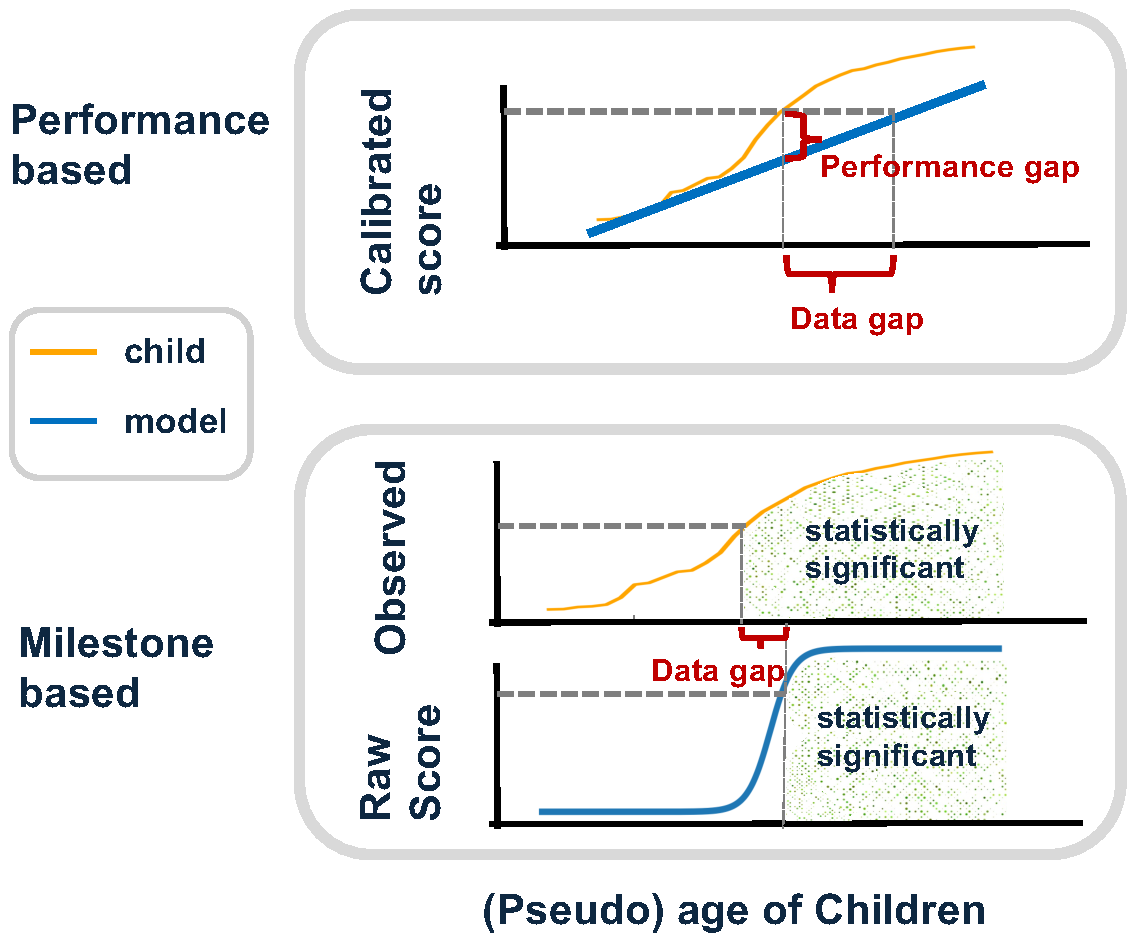
\includegraphics[width=0.92\textwidth]{ch2_literature_review/fig/measure.pdf}
  \caption[Thresholded and graded measures of competence]{Schematic contrast between thresholded and graded evaluation. A milestone analysis treats evidence for a specified competence as present once an explicit statistical criterion is met. A graded analysis retains continuous performance and supports comparison of strength and trajectory. Both depend on the validity of the underlying task.}
  \label{fig:litreview:measures}
\end{figure}

Thresholded evaluation is common in targeted syntactic work. A model is said to exhibit a dependency when it assigns higher probability to the predicted member of a controlled contrast reliably above chance, or when a theoretically specified surprisal interaction is present \citep{linzen2016assessing,marvin2018targeted,Hu2020,PearlSprouse2013}. This formulation clarifies what has been demonstrated: the model has crossed a criterion for one operationally defined construction. It does not imply mastery of syntax more generally, and it does not show that the mechanism producing the effect is the same as a child's. Results can be sensitive to item construction, probability estimation, and the statistical rule used to declare the milestone \citep{warstadt2020blimp,wilcox2023testing}.

Graded evaluation reports accuracy, surprisal, perplexity, correlation, or another continuous score \citep{Warstadt2023,Choshen2024}. Continuous measures preserve differences among checkpoints and architectures, but global improvement can obscure a missing generalization. Perplexity may decrease as frequent sequences become more predictable while a particular long-distance dependency remains absent \citep{Hu2020}. Likewise, reaching or exceeding an adult aggregate score does not establish that every component competence has been acquired.

For child--model comparison, thresholded analyses are most informative when the criterion corresponds to an independently established developmental effect, while graded analyses are most informative when both populations contribute observations on a shared scale or through an explicit linking model. Reporting both is often preferable: a threshold locates the emergence of a theoretically defined behavior, and the continuous effect size describes how it strengthens. Figure~\ref{fig:litreview:measures} illustrates that the two summaries compress different features of the same evidence.

\subsection{Developmental trajectories}
\label{sec:litreview:trajectories}

Endpoint similarity is weak evidence for developmental similarity because different learning routes can converge on the same final score. Trajectory analysis instead evaluates performance across exposure and asks about acquisition order, curve shape, error distribution, and sensitivity to changes in the learning environment \citep{Chang2022,Evanson2023,Ma2024}. It links milestone and graded analyses: milestones identify transitions, while continuous measurements reveal whether change is gradual, abrupt, monotonic, or temporarily regressive.

Lexical work illustrates this approach through neural age of acquisition: the point in training at which the model's evidence for an individual word meets a predeclared criterion. Model acquisition order can then be compared with child age-of-acquisition norms and related to frequency, contextual diversity, and interaction \citep{Chang2022,Ma2024}. The comparison requires care. A checkpoint is an amount of optimization, not a child's chronological age; the mapping becomes meaningful only after accounting for the amount and order of input processed and for repeated exposure across epochs.

Curve shape provides additional evidence. Children sometimes show U-shaped development, producing stored irregular forms correctly, then overgeneralizing a productive rule, and finally recovering the exceptions \citep{Marcus1992}. Related non-monotonic patterns in neural learners are more informative than endpoint accuracy because they constrain the interaction among item frequency, generalization, and memory \citep{michaly2025development}. Still, a visually similar curve is not sufficient. The error types, item-level ordering, exposure scale, and conditions producing the reversal must also agree.

Trajectory analysis also tests whether grammatical phenomena emerge in an order resembling child development. Some model capabilities improve smoothly, whereas others appear more abruptly, and their relative ordering may change with architecture or corpus composition \citep{Evanson2023}. Cross-linguistic work can determine whether the ordering follows proposed processing constraints or merely the statistics of a particular English corpus \citep{constantinescu2024exploring,ficarra2025distributional}. Such comparisons are most useful when age norms are precise and the evaluation remains constant across checkpoints; post-hoc selection of thresholds or checkpoints can manufacture apparent stages.

Finally, a developmental trajectory includes the sequence of experience, not only the cumulative token count. Curriculum learning and interaction may change what is learned at a given budget. Evidence that preserving local discourse continuity can matter more than globally sorting child-directed utterances by child age cautions against equating any ``simple-to-complex'' ordering with the child's curriculum \citep{feng2024child}. Synthetic variation can improve some morphosyntactic outcomes without producing equivalent gains in semantics or pragmatics \citep{haga2024babylm}. Trajectory alignment must therefore be reported per domain rather than reduced to one global developmental score.

\subsection{Measurement uncertainty}
\label{sec:litreview:uncertainty}

Both developmental experiments and model evaluations vary, but their uncertainty enters at different stages. The relevant question is not simply which learner is noisier. It is which components of the observed variance reflect the target knowledge, which reflect the measurement procedure, and which can legitimately be compared.

\begin{figure}[tbp]
  \centering
  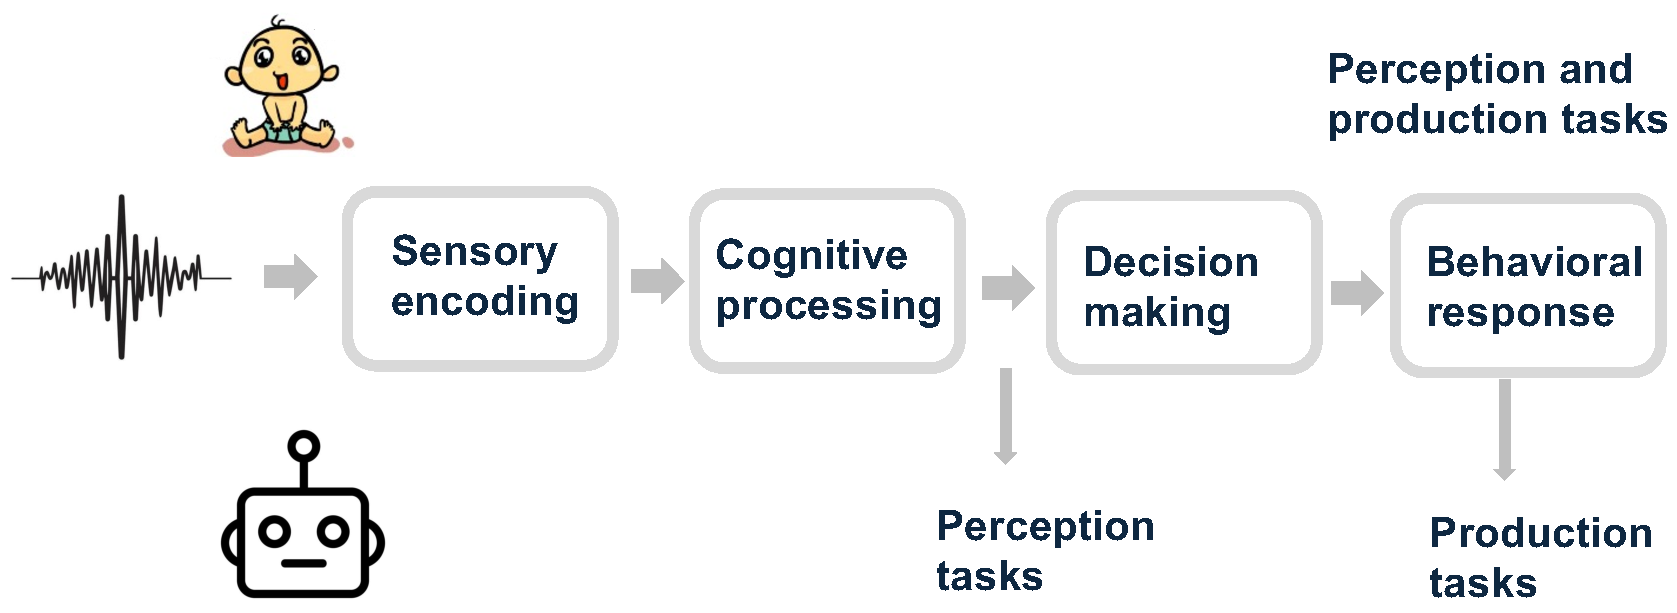
\includegraphics[width=0.92\textwidth]{ch2_literature_review/fig/noise.pdf}
  \caption[Measurement stages in child and model evaluation]{Sources of variation across a simplified evaluation pipeline. Infant and child behavior is observed after sensory encoding, cognitive processing, decision or response selection, and motor execution. Many model perception scores are read from representations through a task model before an overt response stage; generated model output is observed later in the pipeline. The comparison must identify, rather than assume away, these distinct measurement stages.}
  \label{fig:litreview:noise}
\end{figure}

For children, sensory encoding depends on signal quality and hearing; cognitive processing includes the developing representation of interest; decision and response selection depend on arousal, familiarity, memory, and task interpretation; execution adds oculomotor, articulatory, equipment, and coding error. Some variation is nuisance, but some may be developmental signal: inconsistent responding can reflect a transitional representation rather than random failure \citep{Mitchell2022,kucharsky2024habituation}. Large collaborative studies document substantial heterogeneity across laboratories, procedures, ages, and individual infants \citep{ManyBabies2020}. Preferential-looking effects can be robust at the group level while showing limited individual test--retest reliability \citep{Monroy2021,DeBolt2020,byers2022six,schreiner2024limited}.

For models, variability arises from initialization, data order, stochastic optimization, dropout, preprocessing, hardware and numerical nondeterminism, and sampling at inference \citep{Srivastava2014,dodge2020fine,summers2021nondeterminism}. Conditional on a fixed trained model and a deterministic scoring procedure, repeated evaluation of the same input can be identical. That narrow repeatability should not be confused with eliminating model uncertainty. Different seeds may produce materially different learning trajectories, and even a fixed model's apparent competence depends on task-model decisions such as layer, probe, prompt, tokenization, and decoding. These sources are often controllable and estimable, but they are not absent.

The central asymmetry is thus structural. A child's discrimination score is observed after several embodied response stages, whereas an ABX or cosine score may be calculated directly from a selected representation. Production moves model evaluation closer to an overt response, but child articulation and transcription still have no simple analogue in model decoding. Adding arbitrary noise to model outputs does not solve this problem: it can mimic the width of a behavioral distribution without reproducing its causal sources. Likewise, collecting more infant trials reduces sampling error but cannot by itself separate unstable knowledge from state-dependent behavior.

Calibrated analysis should instead propagate uncertainty on both sides. Human estimates should report exclusions, trial counts, coding reliability, individual and laboratory effects, and uncertainty around age-specific means. Model estimates should report independent training runs, checkpoint selection, task-model choices, and item-level confidence intervals. Where possible, the same hierarchical model should estimate stimulus-level and learner-level effects, while preserving the distinction between biological participants and random model instances. This does not make the noise structures identical; it prevents differences in precision from being mistaken for differences in competence.


\section{Input alignment}
\label{sec:litreview:input}

Outcome alignment determines whether the two learners are measured comparably; input alignment determines whether they have been asked to solve comparable learning problems. ``Child-scale'' is not a property of token count alone. Children encounter spoken language in recurring activities, accompanied by visible events, interlocutors, and feedback. The distribution changes with age and with the child's own behavior. A corpus can match one part of this experience while diverging sharply on others. For that reason, input claims should be decomposed into register, modality, interaction, quantity, and temporal organization rather than summarized by a single realism label.

\subsection{Quality, register, modality, and interaction}
\label{sec:litreview:input-quality}

\paragraph{Language-only text.}
Web corpora such as Common Crawl, C4, and Wikipedia provide extensive coverage of lexical, syntactic, and factual patterns \citep{buck2014n,raffel2020exploring,Kaplan2020}. They are nevertheless dominated by written, adult-directed genres: news, reference material, online discussion, and technical prose. Compared with child-directed speech, these sources differ in vocabulary, utterance length, discourse function, repetition, and topic distribution \citep{Huebner2021}. Shuffling documents also removes the contingent sequence in which one conversational turn responds to another. A model trained on this material may answer whether a pattern is learnable from broad written evidence, but not whether it is learnable from the experience available to a young child.

The BabyLM Challenge constrains training to 10 or 100 million words and combines child-directed transcripts with educational and simplified materials \citep{Warstadt2023}. It therefore improves control over both scale and register and makes comparison across architectures possible within a common budget. Its input remains largely textual, however. Transcribed speech omits prosody, voice, timing, overlap, and much of the situational context that makes an utterance interpretable. A developmentally bounded text corpus is thus a valuable experimental resource, but it is not a complete reconstruction of infant input.

Naturalistic child-directed transcripts, especially CHILDES, more closely represent the vocabulary and conversational structure addressed to children \citep{macwhinney_childes_2000}. Child-directed speech tends to contain shorter utterances, concrete and frequent vocabulary, repetition, reformulation, and prosodic adaptation; its composition predicts developmental outcomes \citep{WeislederFernald2013}. The main limitation is not only corpus size. Recordings sample particular families and activities, transcription maps a continuous multimodal exchange into discrete words, and the resulting database does not preserve everything that was perceptually available. ``Training on CHILDES'' should consequently be accompanied by the languages, participants, age ranges, speaker roles, and preprocessing decisions used.

Synthetic augmentation attempts to expand such corpora without returning to adult web register. Paraphrases and variation sets generated from child-directed utterances can increase lexical or syntactic diversity and improve some formal evaluations \citep{haga2024babylm}. But register imitation is not equivalent to interaction. Models generating caregiver-like dialogue can reproduce local lexical and utterance statistics while overstating alignment and failing to reproduce turn-by-turn contingency \citep{LiuFourtassi2024}. Synthetic data are best described by the property they add---paraphrastic variety, simplified syntax, or a target vocabulary---rather than as globally child-like.

\paragraph{Language-only audio.}
Speech supplies information removed by transcription: segmental variation, prosody, speaker identity, timing, and cues to turn and utterance boundaries. These signals are central to phonetic category formation and segmentation \citep{Kuhl2006,Saffran1996}. Read-speech and audiobook corpora offer clean acoustic conditions and relatively reliable annotation, but their adult-directed register and performance style differ from home interaction. Spontaneous adult speech improves discourse naturalness without necessarily matching what is addressed to a child.

Long-form child-centered recordings preserve more of the natural acoustic ecology, including background sound, overlapping voices, changing distance from speakers, and extended daily routines \citep{cristia2020accuracy,bergelson2023everyday}. That realism creates a difficult learning signal: target speech is sparse, noisy, and only partly directed to the child. Systems evaluated on clean audiobooks and on long-form recordings are therefore changing acoustic quality and register together \citep{lavechin2024modeling}. This trade-off is scientifically useful if it is reported explicitly; otherwise, a performance gap can be misattributed to the amount of data or to architecture.

\paragraph{Language with vision.}
Visual context makes referential learning possible in a way that text or audio alone does not. Large image--caption collections such as LAION and COCO provide millions of paired examples \citep{schuhmann2022laion,lin2014microsoft}. Their captions describe images for adult readers rather than participating in a child's unfolding activity. The pairing is curated and static, often identifying a salient object more cleanly than a natural scene would. These resources establish what vision--language architectures can learn from large aligned datasets, but they provide limited evidence about early cross-situational learning.

Synthetic child-directed captions occupy an intermediate position. Developmental vision--language work can pair child-perspective images with simplified descriptions and evaluate grounded combinations on child-oriented tests \citep{Wang2025}. Such data improve register correspondence while retaining a clean supervised pairing. They do not recreate the ambiguity of a caregiver utterance whose referent depends on joint attention, current action, and conversational history.

Egocentric video more directly samples the visual stream available to individual children. SAYCam follows a small number of infants longitudinally and has supported demonstrations of word--referent learning from a single child's visual and linguistic experience \citep{sullivan2021saycam,Vong2024}. BabyView broadens the recording effort and improves visual quality and participant diversity \citep{Long2024}. Yet a head-mounted camera is not an infant's perceptual system: camera field of view differs from gaze and attention, and usable paired speech is far scarcer than web-scale image--text examples. High ecological validity therefore comes with limited coverage and measurement uncertainty of its own.

\paragraph{Language, vision, and social interaction.}
Children learn in exchanges structured by turn taking, joint attention, communicative intention, and contingent caregiver response \citep{Tomasello1995,Csibra2009}. Dyadic corpora retain some of this structure. Shared book-reading recordings combine caregiver and infant perspectives in a constrained but genuinely interactive setting \citep{ahamat2025shared}; ECOLANG annotates speech, gesture, and gaze in interactions with older children \citep{gu2025ecolang}; and game-based corpora extend multimodal dialogue to middle childhood \citep{bodur2021chico,goumri2024chica}. Their value lies in temporal coordination across channels, not merely in the coexistence of audio and video.

These corpora remain too small and specialized to serve as drop-in replacements for large language-model training sets. They can instead support focused learning experiments, evaluation of contingent behavior, or estimation of the distributions that a larger simulation should preserve. Treating every audiovisual recording as ``social'' would erase the key distinction: co-occurrence presents signals together, whereas interaction makes one participant's behavior conditional on the other's.

\begingroup
\scriptsize
\setlength{\tabcolsep}{3pt}
\setlength{\LTleft}{0pt}
\setlength{\LTright}{0pt}
\begin{longtable}{@{}p{0.14\textwidth}p{0.18\textwidth}p{0.20\textwidth}p{0.24\textwidth}p{0.18\textwidth}@{}}
\caption[Representative input resources for developmental modeling]{Representative input resources organized by modality, register, interactional structure, and principal limitation. The entries characterize resource types and do not imply that every study uses identical preprocessing.}\label{tab:litreview:input-resources}\\
\toprule
\textbf{Resource} & \textbf{Modality and register} & \textbf{Interactional structure} & \textbf{Developmental value} & \textbf{Principal limitation} \\
\midrule
\endfirsthead
\multicolumn{5}{@{}l}{\small Table~\ref{tab:litreview:input-resources} continued}\\
\toprule
\textbf{Resource} & \textbf{Modality and register} & \textbf{Interactional structure} & \textbf{Developmental value} & \textbf{Principal limitation} \\
\midrule
\endhead
\midrule
\multicolumn{5}{r@{}}{\small Continued on next page}\\
\endfoot
\bottomrule
\endlastfoot
Common Crawl \citep{buck2014n} & Written, mostly adult-directed web text & Documents rather than interaction & Broad lexical and domain coverage & Register, scale, and temporal mismatch \\
C4 \citep{raffel2020exploring} & Filtered written web text & Documents rather than interaction & Reproducible large-scale LM training & Adult-written genres and weak grounding \\
BabyLM \citep{Warstadt2023} & Mixed text with child-directed and simplified components & Some dialogue after transcription & Controlled 10M/100M-word budgets & Predominantly textual; heterogeneous sources \\
CHILDES \citep{macwhinney_childes_2000} & Transcribed child-directed and child speech & Natural conversational turns & High register correspondence across languages & Sparse sampling and loss of acoustic/visual context \\
Synthetic CDS variation sets \citep{haga2024babylm,LiuFourtassi2024} & Generated child-directed-style text & Simulated turns or paraphrases & Scalable control of surface register & Limited contingency and inherited generator bias \\
Read-speech collections \citep{Lavechin2023BabySLM} & Clean adult-directed audio & Narration rather than dialogue & Acoustic and prosodic learning at scale & Low interactional and register correspondence \\
Child-centered long-form audio \citep{cristia2020accuracy,bergelson2023everyday} & Naturalistic home audio & Extended daily interaction & Realistic acoustic ecology and exposure estimates & Noise, overlap, privacy, and sparse annotation \\
LAION \citep{schuhmann2022laion} & Web image--text pairs & No contingent interaction & Large-scale visual grounding & Adult web captions and curated pairing \\
COCO \citep{lin2014microsoft} & Curated images and descriptive captions & No contingent interaction & Controlled object and scene descriptions & Captioning task unlike child-directed talk \\
Developmental synthetic captions \citep{Wang2025} & Child-oriented text with visual scenes & Static pairing & Register-controlled grounded evaluation & Generated language and absent joint attention \\
SAYCam \citep{sullivan2021saycam,Vong2024} & Infant-perspective video with speech & Naturalistic home activity & Longitudinal, child-specific grounding & Few children and camera--attention mismatch \\
BabyView \citep{Long2024} & Egocentric developmental video and audio & Naturalistic activity & Broader and higher-quality child-perspective sampling & Modest scale relative to web corpora \\
Shared book reading \citep{ahamat2025shared} & Dyadic audiovisual child-directed speech & Turn taking and joint attention & Aligned caregiver and infant perspectives & Narrow activity and small sample \\
ECOLANG \citep{gu2025ecolang} & Speech, gesture, and gaze & Naturalistic dyadic interaction & Explicit cross-channel coordination & Older age group and limited training scale \\
CHICO/CHICA \citep{bodur2021chico,goumri2024chica} & Multimodal task dialogue & Collaborative word games & Naturalistic communicative adaptation & Task- and age-specific interaction \\
\end{longtable}
\endgroup

\subsection{Quantity and temporal organization}
\label{sec:litreview:input-quantity}

Claims about data efficiency require a defined denominator. Studies variously report words, subword tokens, utterances, audio hours, image--text pairs, gradient updates, or epochs. These units do not convert transparently. One hour of long-form audio contains silence, distant speech, overlapping speakers, and utterances not directed to the child; one hour of an audiobook is densely linguistic. Likewise, a word processed during a hundredth epoch is not equivalent to a newly encountered word in a new situation. Reporting a nominal corpus size without total presentations and sampling procedure can therefore make a heavily recycled training regime appear child-scale.

Estimates of children's cumulative linguistic exposure vary with recording method, socioeconomic and cultural context, the definition of speech addressed to or merely audible to the child, and extrapolation from sampled days \citep{hart1992american,WeislederFernald2013,Frank2023}. A defensible comparison should state a range and sensitivity analysis rather than a single universal number. It should also distinguish raw exposure from \emph{effective exposure}: what the learner can encode given signal quality, attention, vocabulary, and multimodal context.

\paragraph{Fixed-corpus trajectories.}
In a fixed-corpus design, one dataset is repeated while the model is evaluated across checkpoints \citep{Chang2022,Evanson2023,Ma2024}. Holding composition constant helps isolate learning dynamics and makes frequent measurement inexpensive. It is useful for studying item acquisition order and the emergence of particular generalizations. But the developmental analogy is limited. Children do not receive the same closed corpus in a new random order on every pass; their vocabulary and activities expand, interlocutors respond to them, and old events cannot be replayed exactly.

Repeated epochs also change the effective quantity. A model trained for 100 epochs over ten million words has processed one billion word presentations, even though its unique corpus is described as ten million words. Memorization, overtraining, and declining lexical novelty may shape the resulting trajectory. At minimum, studies should report unique tokens, total token presentations, number of epochs, sampling with or without replacement, and the exposure count at every evaluated checkpoint.

\paragraph{Successive scaling.}
Scaling designs train otherwise comparable models on increasingly large samples and ask how much input is needed for a target behavior \citep{warstadt2020learning}. BabyLM makes this comparison explicit within bounded text budgets \citep{Warstadt2023,Hu2024}; STELA and BabySLM extend related logic to quantities and registers of speech \citep{Lavechin2023BabySLM,lavechin2024modeling}. The input level at which a model crosses a milestone can be compared with a plausible exposure range for children.

This design better represents cumulative amount, but independent models do not form a longitudinal learner. Each scale may begin from a new initialization, and the larger training set is not necessarily an ordered extension of the smaller one. Apparent movement along a learning curve can therefore combine data quantity, sample composition, and between-run variation. Nested corpora, multiple seeds per scale, and identical evaluation make the interpretation stronger.

\paragraph{Curriculum and continual learning.}
Children's input is incrementally arriving and contextually clustered. A caregiver repeats a topic within an exchange, adapts utterances to a response, and introduces new vocabulary through changing activities. Curriculum experiments attempt to preserve selected parts of that structure. Globally ordering child-directed speech by the child's age has not consistently improved model outcomes, while keeping local conversational context can matter \citep{feng2024child}. The relevant curriculum may therefore lie in coherent interaction rather than a simple global ordering from short to long sentences.

Continual learning offers the closest formal analogy to an accumulating stream: the model updates on new data while retaining what it learned earlier. Standard neural systems are vulnerable to catastrophic forgetting, in which new learning disrupts earlier representations \citep{mccloskey1989catastrophic}. That failure is not merely an inconvenience to be hidden by replay. It identifies a property---stable integration of new evidence with long-term knowledge---that a developmental model must explain. Replay buffers, retrieval, and external memory can be tested as hypotheses, but their stored amount should count toward the model's effective exposure.

No current design aligns quantity, lexical novelty, temporal order, interaction, and learning continuity simultaneously. Fixed corpora maximize experimental control but recycle a static distribution; successive scaling improves amount calibration but often substitutes different learners for developmental time; continual learning represents sequential arrival but introduces retention problems. The appropriate choice depends on the claim. Studies should state which dimension is controlled and which remains an abstraction.


\section{Implications, reporting standards, and thesis research gaps}
\label{sec:litreview:implications}

\subsection{What a calibrated comparison licenses}
\label{sec:litreview:inference}

Input and outcome alignment are distinct requirements. Strong outcome alignment with weak input alignment shows that a model can reproduce a behavioral contrast under a different learning regime. Strong input alignment with weak outcome alignment shows what representations or engineering scores arise from child-oriented data, but not whether child behavior has been reproduced. When both are reasonably aligned, model success supports a bounded sufficiency claim: the specified learner can acquire the specified outcome from the specified experience. Even then, success does not establish that children use the same internal mechanism.

This framework separates two legitimate research orientations. Developmentally oriented modeling uses a model to test hypotheses about learning and therefore requires calibrated input and outcomes. Engineering-oriented evaluation uses human performance to diagnose or improve artificial systems; it can be scientifically valuable without recreating development, but its results should not be presented as evidence about how children learn. Problems arise when the orientation changes between method and conclusion---for example, when a web-trained model's benchmark success is interpreted as a developmental proof, or when failure under a mismatched task is treated as evidence for an innate human constraint.

Model failure becomes informative through controlled contrasts. If input and evaluation are fixed while memory architecture changes, a performance difference can bear on the role of memory. If architecture and task are fixed while register changes, the comparison can isolate properties of the input distribution. If all dimensions vary at once, attribution is impossible. Calibration is therefore not a demand that every model imitate a child in every respect; it is a discipline for identifying which difference is the experimental variable.

\subsection{Minimum reporting for interpretable evidence}
\label{sec:litreview:reporting}

Transparent reporting should make the inferential chain reconstructible. At a minimum, a developmental model comparison should specify:

\begin{enumerate}
  \item \textbf{The orientation and claim.} State whether the study tests developmental sufficiency, mechanism, prediction of human behavior, or engineering performance, and formulate the conclusion at the same level.
  \item \textbf{The input population.} Report language, register, speaker roles, child ages, modality, activity or genre, collection procedure, filtering, deduplication, and synthetic-data provenance.
  \item \textbf{The exposure budget.} Give unique and total tokens or hours, epochs, sampling and curriculum, amount processed at each checkpoint, and a justified range for the human comparison.
  \item \textbf{The outcome and task model.} Identify the construct, stimuli, response alternatives, prompt or probe, selected layer, scoring rule, threshold, and the linking assumption between child and model measures.
  \item \textbf{The developmental comparison.} Predefine the human age range, checkpoints, acquisition criterion, and whether evidence concerns endpoint, order, curve shape, or item-level errors.
  \item \textbf{Uncertainty and robustness.} Report participant exclusions and measurement reliability for humans; seeds, runs, numerical settings, checkpoint selection, and decoding for models; provide item- and learner-level uncertainty where possible.
  \item \textbf{Residual mismatches.} Name the missing modalities, interaction, cognitive resources, or response stages and state how they limit the conclusion.
\end{enumerate}

The checklist does not require every study to solve the entire calibration problem. It requires enough detail to know which problem was solved. Standardized benchmarks remain useful, but their scores should be accompanied by developmental task analyses. Naturalistic corpora remain useful despite incomplete coverage, but their sampling and preprocessing must be visible. Cumulative evidence emerges when later work can reproduce both the learner and the comparison, not only the final score.

\subsection{Research gaps addressed in this thesis}
\label{sec:litreview:thesis-gaps}

The review identifies three connected gaps that motivate the empirical chapters that follow. First, lexical development lacks a production-oriented measure that aligns model generation with the cumulative growth recorded for children while making input budgets explicit. Chapter~\ref{chp2_chap} addresses this gap with \textsc{corpus-CDI}, comparing the expressive vocabularies of children and language models across developmental stages and controlled exposure. This operationalizes the present chapter's argument that a vocabulary count is meaningful only when observation opportunities, lexical units, and developmental time are defined jointly.

Second, differences between child and model syntax may reflect memory and lexical exposure rather than grammatical representation alone. Chapter~\ref{chp3_chap} tests whether episodic retrieval changes language models' sensitivity to syntactic minimal pairs and whether it reduces a lexical-frequency gap. Retrieval is thereby treated as a controlled architectural hypothesis under a common outcome measure, rather than invoked after the fact to explain a mismatch.

Third, existing child-oriented corpora preserve linguistic register more readily than interactional contingency. Chapter~\ref{chp4_chap} evaluates how well large language models reproduce child--caregiver dialogue and then isolates which forms of caregiver feedback support grammar learning. The benchmark distinguishes surface resemblance from turn-level behavior, while the learning experiment treats feedback as an input variable. Together, these studies address the interactional component of input alignment that static corpora leave unresolved.

These contributions do not attempt to build a globally child-equivalent learner. They make narrower comparisons in which the inputs, outcomes, or hypothesized mechanisms can be varied and measured. Their conclusions should therefore be read as evidence about lexical growth, episodic retrieval, and caregiver feedback under the stated conditions, not as a general equivalence between children and contemporary language models.

\subsection{Limits of the framework}
\label{sec:litreview:limits}

Calibration is necessary for developmental interpretation but not sufficient for mechanistic identity. Two systems can receive similar observable input and produce similar responses while relying on different internal representations. Stronger mechanistic evidence requires intervention, process-level prediction, and generalization to new tasks, not only behavioral correlation \citep{Marr1982,Perfors2011}.

The framework also abstracts over individual and cultural variation. Children's environments differ in quantity, interlocutors, activity structure, multilingual exposure, and the social organization of learning \citep{WeislederFernald2013,bergelson2023everyday}. Average developmental curves can conceal distinct routes and can make one narrowly sampled corpus appear universal. Model ensembles are not replicas of this variation because their differences arise from initialization and training rather than lived environments. Future comparisons should link individual input histories to individual outcomes where the data permit.

Finally, the evidence base is uneven. Phonological and lexical perception have established infant paradigms, syntactic model evaluation has extensive minimal-pair resources, and word--referent matching provides a promising shared task. Naturalistic production, multimodal sentence meaning, and socially grounded pragmatics remain less well aligned. The selective study maps in this chapter represent that imbalance rather than a complete quantitative review, and claims about gaps should be updated as new corpora and matched paradigms become available.


\section{Chapter summary}
\label{sec:litreview:summary}

Computational models can inform language acquisition when the comparison is calibrated to the inference being made. Outcome alignment requires more than a shared linguistic label: child and model tasks must target the same construct through stimuli, response alternatives, and measures whose relationship is explicit. Thresholded tests, graded scores, developmental trajectories, and uncertainty each reveal different aspects of learning. They should be combined where possible rather than treated as interchangeable summaries.

Input alignment is similarly multidimensional. A child-oriented token budget does not compensate for adult-written register, and naturalistic child-directed language does not automatically preserve perceptual modality or social contingency. Repeated epochs, shuffled corpora, successive scaling, and continual learning embody different assumptions about developmental time. Consequently, every success and failure must be indexed to the quantity, quality, ordering, and interactional structure of the experience that produced it.

The strongest conclusion supported by an aligned success is a conditional sufficiency claim: a particular learner can acquire a particular outcome from a particular input. Mechanistic conclusions require additional controlled variation and process-level evidence. This bounded logic guides the chapters that follow, which examine lexical growth under defined exposure, episodic retrieval under shared syntactic outcomes, and caregiver interaction as a structured component of the learning environment.
